\documentclass{beamer}
\usetheme{Copenhagen}
\usepackage{graphicx}
% \usepackage[ruled,vlined,english]{algorithm2e}
% \renewcommand{\thealgocf}{}
% \usepackage{hyperref}


\author[Jumeau numérique: Environnement]{\large Hanna CHETOUANE, Narmimane ZAOUACHE \\ \vspace{-0.8cm} \date{\today}}
\title[Microclimat urbain]{\textbf{Jumeau numérique dans l'environnement:} \\ Microclimat urbain}



\begin{document}

\begin{frame}
    \titlepage
    \vspace{-0.4cm}
    \begin{center}
        UFR of Mathematics and Informatics - University of Strasbourg 
        \\[0.2cm] 
        \textit{Comment les jumeaux numériques aident-ils à comprendre les effets des aménagements urbains sur le micro-climat ?}
    \end{center}
\end{frame} 


\begin{frame}{Plan}
    \tableofcontents    
\end{frame}


\begin{frame}{Contexte}
    \small
    \begin{itemize} % plus développer ?
        \item L'écologie et le climat sont devenus des enjeux majeurs, surtout dans les villes où se développent des îlots de chaleur
        \item Solutions: Végétalisation, choix de matériaux adaptés et aménagements urbains repensés
        \item Les collectiviités locales doivent ainsi prendre des décisions sur les stratégies d'aménagement à adopter et en évaluer l'impact environnemental et sanitaire
    \end{itemize}
    $\rightarrow$ Simuler et prédire ces effets de ces choix sur le microclimat urbain et la santé publique $\Rightarrow $ \textbf{Jumeau numérique}
\end{frame}


\begin{frame}{Qu'est-ce qu'un jumeau numérique ?}
    \small
    \begin{itemize}
        \item Réplique virtuelle et dynamique d'un système réel, qui, couplé à des outils de simulation, permet d'analyser et prédire son comportement dans différentes conditions
        \item S'appuie sur des données réelles (météorologiques et urbaines) issues de capteurs, d'observations ou de modèles physiques
    \end{itemize}
    \begin{center}
        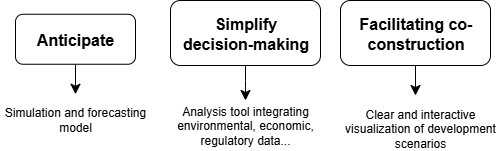
\includegraphics[width=0.7\textwidth]{images/objectifs_jm.png} \\
    \end{center}
    Défi actuel en France: projet JNFT porté par l'IGN, le Cerema et l'Inria, qui vise à créer un jumeau numérique multithématique couvrant le territoire français
\end{frame}


\begin{frame}{Fonctionnement d'un jumeau numérique} %Architecture et pipeline}
    \hspace*{-0.5cm}
    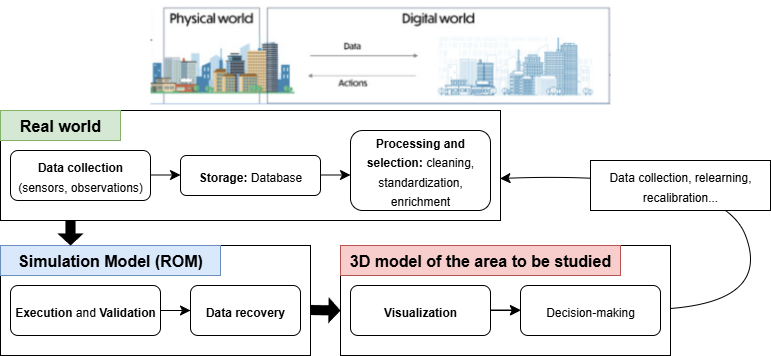
\includegraphics[width=1.1\textwidth]{images/pipeline.png} \\
\end{frame}


\begin{frame}{Méthodes}
    %Modélisation de phénomènes physiques
    \textbf{Physique $\rightarrow$ numérique:}  \\
    Données (météo, propriétés des matériaux, composition de l'air) $\rightarrow$ paramètres \hspace{1cm}  Zone d'étude $\rightarrow$ Maquette 3D maillée % pour résoudre numériquement par FEM, VM, DM
    \textbf{Modèles physiques:}
    \begin{itemize}
        \item Phénomènes physiques continus (exemple): PDEs (Navier-Stockes, chaleur, transport, diffusion)
        \item Interaction entre batiments, vent, végétation: Fluid-Structure Interaction (NS + Elasticity)
        \item Ecoulement d'air et échanges thermiques: Computational Fluid Dynamics (NS + Heat; Transport; transfert radiatif) % effet du soleil sur les façades
    \end{itemize}

    % résolution très lourde et longue à calculer, donc:
    \textbf{Utilisation ROM:} Réduction de l'ordre des modèles physiques pour accélérer les simulations 
    \textbf{Offline:} Préparation du modèle
    \begin{itemize}
        \item Réduction de la dimension en capturant l'essentiel du système: Proper Orthogonal Decomposition (POD), Reduced Basis Method (RBM)
        \item Hyper-réduction: Réduit temps de calcul des termes non-linéaires (DEIM, gappy POD) % en évaluant seulement certains points clés du modèle
                                                        % DEIM: Discrete Empirical Interpolation Method; gappy POD: gappy Proper Orthogonal Decomposition
    \end{itemize}
    \textbf{Online:} Simulation du modèle réduit pour tester différents scénarios rapidement

    \textbf{Data-Driven Models:} basé sur les données, prédiction rapide % sur le micro-climat
    \begin{itemize}
        \item Régression: prédit des phénomènes (température, qualité de l'air, vent) à partir de variables (matériaux, végétation...) 
        \item Gaussian Process: prédit et donne l'incertitude pour des zones avec peu de données
        \item Réseaux de Neuronnes: capture les relations complexes et non-linéaires entre les variables 
        \item Modèles d'ensembles: amélioration de la précision et de la robustesse des prédictions, en combinant plusieurs modèles
    \end{itemize}

    \textbf{Data assimilation:} Combinaison des modèles physiques et des données pour corriger les simulations, obtenir un maximum de précision et rendre ces simulations exploitables % pour la prise de décision
    \begin{itemize}
        \item VAR: ajuste le modèle physique pour que les simulations collent aux observations (sur un ou plusieurs pas de temps)
        \item Filtre de Kalman: Mise à jour des prédictions en temps réel pour un suivi dynamique
        \item PBDW, GEIM: reconstruction du système avec peu de données, pour une vue d'ensemble
        \item Capteurs virtuels: estimation de variables où il n'y a pas de mesures, voir l'effet de nouveaux aménagements
    \end{itemize}

\end{frame}


\begin{frame}{Données et instrumentation}
    % tableau
\end{frame}


\begin{frame}{Vérification et validation / UQ}
    
\end{frame}


\begin{frame}{Transfert et déploiement}
    
\end{frame}


\begin{frame}{Perspectives et limites}
    
\end{frame}


\begin{frame}{Bibliographie}
    % https://www.ign.fr/institut/un-jumeau-numerique-de-la-france-pour-piloter-la-transition-ecologique
    % https://cnig.gouv.fr/IMG/pdf/2025.01_20_jnft_presentation_cnig_pole_territoires.pdf
    % Fondateurs de la démarche: IGN, Cerema, Inria
    % slide 10 -> 30% pour les aménagements durables
    % https://www.sciencedirect.com/science/article/pii/S2212095525002469
\end{frame}



\end{document}